In this paper, we propose a Multistream Domain Adaptation (MSDA) framework to address the major issues in our problem setting. 
% \textcolor{red}{To be specific, the assumption of heterogeneous domains holds valid between source and target streams,
% while there are concept drift in both streams as well. Thus, our goal of designing this framework is to use as much information as possible from the source stream,
% to predict the instance labels in the target stream. [there's no reason to restate the problems/goals right after you stated them]}
To achieve this goal, we establish a framework with the following modules:

\begin{enumerate}
\item A domain adaptation module that helps find an optimized latent subspace for both source and target streams. 
\item A concept drift detection module that detects concept drift in both source and target streams.
\end{enumerate}

\begin{figure}[t]
\centering
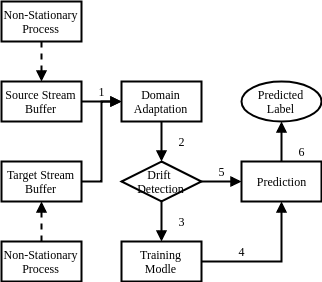
\includegraphics[width=0.7\columnwidth]{Figures/flowchart.png}
\caption{Multistream Classification with Domain Adaptation}
\label{fig:flowchart}
\end{figure}

Applying these two modules together, once a concept drift is detected, we use data instances from both streams in the most recent window to update the feature mapping, so that the domain adaptation problem can be addressed. The diagram of this algorithm can be found in Figure \ref{fig:flowchart}.

In our framework, data instances are generated simultaneously from both source and target domains. The content in parentheses correspond to contents in Figure~\ref{fig:flowchart} and Algorithm~\ref{alg::overall} respectively.

First, a domain adaptation module is triggered to learn projection functions for both source and target data instances (step 1, 2 \& line 2-6). 
Newly arriving instances are transformed to latent feature representation accordingly (line 8-11). 
Second, the change point detection module detects if there is a significant change in either source or target streams within the sliding windows  
Third, once a change point is detected, new classifiers are trained based on these two buffers from $B_s$ and $B_t$ (step 3 \& line 12-16).
Finally, the newly updated classifiers are used to  predict the labels of adapted data instances from target stream $T$ (step 4, 5, 6 \& line 17-18). Details of our proposed method is as follows.

\begin{algorithm}[t]  
\caption{MSDA Algorithm}  
\label{alg::overall}  
\begin{algorithmic}[1]  
\Require  
Labeled source stream $S$,
Unlabeled target stream $T$,  
The size of sliding window $N_m$.
Similarity parameter $\beta$.
\Ensure  
Labels predicted on $T$.
\State /* Initialization */
\State $B_s, B_t \gets readData(S,T)$
\State /* DA for initial buffer */
\State $W_s, W_t \gets genProjectionFunction(B_s, B_t, \beta)$
\State $L_s, L_t \gets genProjectionMatrix(B_s, B_t, W_s, W_t)$
\State $M \gets buildModel(L_s, Y_s)$

\While {$S$ or $T$ $exists$}
\State $B_s, B_t \gets readData(S,T)$
\State /* DA for stream buffer */
\State $W_s, W_t \gets genProjectionFunction(B_s, B_t, \beta)$
\State $L_s, L_t \gets genProjectionMatrix(B_s, B_t, W_s, W_t)$
% \State $M \gets buildModel(L_s, Y_s)$
\State /* Concept drift detection and correction */
\State Call $ChageDetection$ // Algorithm 2
\If {$ChangeDetection = True$}
\State /* Update prediction model */
\State $M \gets buildModel(L_s, Y_s)$

\EndIf
\State /* Generate predictions */
\State $\hat{y_{t}} \gets getPrediction(M,L_t)$
% \State print $getMAE (\hat{y}_t, B_t)$
\EndWhile

\end{algorithmic}  
\end{algorithm}

\subsection{Initialization and Domain Adaptation}

In our proposed framework, instances from source and target streams are stored in $B_{s}$ and $B_{t}$ respectively. 
Recalling our problem setting, data in $B_{s}$ have true labels, while data in $B_t$ come without true labels. 
The domain adaptation method is indeed a optimization problem solved by feature embedding~\cite{shi2010transfer}.
Also, for computational purposes, we design our approach in a way that buffer size in both source and target streams are the same, which means the numbers of data instances in processing window for source and target streams are identical. 
Thus, given a certain time $t$, data that we have are: source stream window matrix $B_s \in \mathds{R}^{N_m \times m}$; source stream window labels vector $Y_{s} \in \mathds{R}^{N_m \times 1}$, and; target stream window matrix $B_t \in \mathds{R}^{N_m \times n}$. 
In this case, the best projection strategy of $L_{s}$ and $L_{t}$ in the latent feature space would be the minimization of following objective function:
\begin{equation}
\label{fcn:overallMinimization}
    \mathcal{O} = \min_{L_{s}, L_{t}}\ell\left ( B_s, L_{s} \right ) + \ell\left ( B_t, L_{t} \right ) + \beta \mathbf{D}\left(L_{s}, L_{t} \right )
\end{equation}
where $\ell\left(\cdot , \cdot \right)$ is a distance function that evaluates the differences between the original data and projected data. 
$\mathbf{D}\left(\cdot, \cdot\right)$ is the co-regularizer that promotes the similarities between the two projected domains ($L_{s}$ and $L_{t}$). $\beta$ is a parameter that determines how desirable the two projected data are similar.
The first two terms are expected to preserve the structure of the original data as much as possible. 
Therefore, we define the loss function $\ell\left(\cdot, \cdot\right)$ as the Frobenius norm, which can also be expressed as a matrix trace norm $\ell\left(B_s, L_{s}\right) $ equals $\left \| B_s - L_{s}W_{s}  \right \|_{F}^2$, and $\ell\left(B_t, L_{t}\right)$ equals $ \left \| B_t - L_{t}W_{t}  \right \|_{F}^2$.

We factorize the original data into projections ($L_{s}$ and $L_{t}$) by linear mapping functions ($W_{s}$ and $W_{t}$).
Also, note that here we are not applying the alternative definition such as $\ell\left(B_s,L_{s}\right) $ as $\left \| B_{s}W_{s} - L_{s}  \right \|_{F}^2$, since this definition will always lead to a trivial solution $W_{s} = 0$ and $L_{s} = 0$, thus $B_{s}W_{s} = L_{s} = 0$ will always minimize the objective function. From Equation~\ref{fcn:overallMinimization} the projected data should preserve the structures of original data.

Furthermore, we define $\mathbf{D}\left(L{s}, L_{t}\right)$ as follows:
\begin{equation}
\label{fcn:crossSimilarity}
    \mathbf{D}\left(L_{s}, L_{t}\right) =\frac{1}{2}\left(\ell\left(B_s, L_{t}\right) + \ell\left(B_t, L_{s}\right)\right)
\end{equation}
which is the mean value of cross-similarity between the original data and projected data. Finally, the parameter $\beta$ controls the trade-off of importance of semantic similarity co-regularization by minimizing the differences between $\mathbf{D}(L_{s}, L_{t})$.

Combining Equation \ref{fcn:overallMinimization} and \ref{fcn:crossSimilarity} together, we obtain the overall optimization objective function as follows:
\begin{equation}
\label{fcn:finalObjectiveFunction}
\begin{split}
    \mathcal{O} &= \left \| B_s - L_{s}W_{s}  \right \|_{F}^2 + \left \| B_t - L_{t}W_{t}\right \|_{F}^2 \\
    &+ \frac{1}{2}\beta \left \| B_s - L_{t}W_{s}  \right \|_{F}^2 + \frac{1}{2}\beta \left \| B_t - L_{s}W_{t}\right \|_{F}^2
\end{split}
\end{equation}
% \textcolor{red}{[you maybe should expand $l(\cdot,\cdot)$ in this equation]}
Notice here the projection itself will perform rotation and scaling on the target matrix to minimize the difference.
Since $L_s$ and $L_t$ are orthogonal matrices, $B_{s}^{\top}B_{s}=1$. Also, we are applying the cyclic permutation property of trace. Thus, Equation \ref{fcn:finalObjectiveFunction} can be expanded by the representation of trace.

We therefore adopt an alternative formula to solve this problem by iteratively fixing one of the projection matrices until the remaining one converges. 
That is, we can take the derivative of $\mathcal{O}$ with regard to $W_s$ and $W_t$.
Under this conditions, our formula is defined as follows accordingly.

\begin{equation}
\begin{split}
    \frac{\partial \mathcal{O}}{\partial W_{s}} =  (2+\beta)W_{s} -2L_{s}^{\top}B_{s} - \beta L_{t}^{\top}B_{t} \\
    \frac{\partial \mathcal{O}}{\partial W_{t}} =  (2+\beta)W_{t} -2L_{t}^{\top}B_{t} - \beta L_{s}^{\top}B_{t} \\
\end{split}
\end{equation}

According to Long et al.~\cite{long2008general}, setting both partial derivatives to zero would generate the optimal solution based on KTT conditions.
Consequently, the projection function for both source and target stream can be formulated as:

\begin{equation}
\begin{split}
    W_s = \cfrac{\beta}{2+\beta} L_{t}^\top B_{s} + \cfrac{2}{2+\beta} L_{s}^\top B_{s} \\
    W_t = \cfrac{\beta}{2+\beta} L_{s}^\top B_{t} + \cfrac{2}{2+\beta} L_{t}^\top B_{t} \\
\end{split}
\end{equation}

After the steps described above, the optimal projection for both source and target stream to the latent feature space would be formed accordingly. 

% Furthermore, we need to screen the optimization to avoid mappings between two totally unrelated data. A sample selection algorithm is used to eliminate those unrelated examp/les, that is, if the source data is too different from target data, we will consider that it is ``too risky'' to conduct the domain adaptation.

%%%%%%%%%%%%%%%%%%%%%%%%%%%%%%%%%%%%%%%%%%%
% Here goes Tao's code
%%%%%%%%%%%%%%%%%%%%%%%%%%%%%%%%%%%%%%%%%%%

\subsection{Classification Module}

Initially, we train a classifier using a small set of data instances from both $S$ and $T$, which are referred to as the initialization data. The new data representation is obtained by using initialization data from $B_s$ and $B_t$ as follows:

\begin{equation}
\begin{cases}
L_s^{(i)}=B_s^{(i)}W_s^{-1} \qquad B_s^{(i)}\in B_s \\
L_t^{(j)}=B_t^{(j)}W_t^{-1} \qquad {B}_t^{(j)}\in {B}_t\\
\end{cases}
\end{equation}

There are several algorithm can be used in MSDA. As new instances arrive in $S$ or $T$, the classifier is updated if there is a drift to ensure that it represents the current concepts. A new classification model is trained using data in $B_s$ and $B_t$ at that time. Concept drift detection and the updating method used by MSDA will be discussed Section~\ref{sec:changedetection} in this section. MSDA predicts the  class label of an incoming target instance from the target stream after projecting the instance into the new data format.


\subsection{Change Detection Module (CDM)}
\label{sec:changedetection}

Previous work~\cite{chandra2016adaptive} of multistream classification uses prediction confidence to detect changes in distribution between two different time windows. Due to possible asynchronous concept drifts between source and target streams, an ensemble of classifiers is maintained and updated if a concept drift is detected in either of these streams of data. Therefore, complex ensemble algorithms may lead to very slow execution.

\begin{algorithm}[t]  
\caption{ChangeDetection: Change Detection}  
\label{alg::detection}  
\begin{algorithmic}[1]  
\Require  
Source instances $B_s=\{B_s\}^{i=1}$, target instances $B_t=\{B_t\}^{j=1}$, new instance $x$, initial mean discrepancy $Disc$, the change parameter $\tau$.
\Ensure  
$True$ if drift is detected, else $False$.
\State /* Instance is from source stream */
\If {$x \in S$}
\State $B_s^{(N_m+1)} \leftarrow x$.
\State $L_s^{(N_m+1)}=xW_s^{-1}$.
\State $B_s^{(i)} \leftarrow B_s^{(i+1)}, i=1,...,N_m$.
\State $L_{s}^{(i)} \leftarrow L_{s}^{(i+1)}, i=1,...,N_m$.
\State $\mu_S=\frac{1}{N_m} \sum_{i=1}^{N_m}  L_{s}^{(i)}W_s^{-1}$.
\State Go to line 16.
\EndIf
\State /* Instance is from target stream */
\State $B_t^{(N_m+1)} \leftarrow x$.
\State $L_{t}^{(N_m+1)}= xW_t^{-1}$.
\State $B_t^{(i)} \leftarrow B_t^{(j+1)}, j=1,...,N_m$.
\State $L_{t}^{(j)} \leftarrow L_{t}^{(j+1)}, j=1,...,N_m$.
\State $\mu_T=\frac{1}{N_m} \sum_{j=1}^{N_m} \mathbf L_{t}^{(j)} W_t^{-1}$.
\State /* Calculate the mean discrepancy $Disc_t$ at time $t$: */
\quad $Disc_t=\|\mu_s^t-\mu_t^t\|^2$.
\State $s=ln\frac{Disc_t}{Disc_0}$.
\State \bf{Return} $s>-ln(\tau)$.
\end{algorithmic}  
\end{algorithm}

We adopt the Maximum Mean Discrepancy (MMD) as the distance measure to compare different distributions. The distance between two distributions can be computed between the sample means of the two domains in the $k$-dimensional embeddings:
\begin{equation}
\begin{split}
&Disc(L_{newS},L_{newT})\\
&= \left\lVert \frac{1}{N_m}\sum_{i=1}^{N_m}  L_s^{(i)} W_{s}^{-1} - \frac{1}{N_m}\sum_{j=1}^{N_m}  L_t^{(j)} W_{t}^{-1}\right\rVert ^2
\end{split}
\end{equation}
where $L_{newS}$, $L_{newT}$ are the set of projected data points in the source and target windows.

We invoke a simple but efficient change detection method by monitoring significant changes in $B_s$ and $B_t$. Since data continuously arrives in the source and target streams, the MMD model in Equation needs to be updated also by updating the mean of adapted data points in the two windows respectively. The online updating process is given by:
\begin{equation}
\begin{cases}
L_s^{(i)}=B_s^{(i+1)}W_s^{-1} \qquad B_s^{(i)}\in B_s \\
L_t^{(j)}=B_t^{(j+1)}W_t^{-1} \qquad {B}_t^{(j)}\in {B}_t\\
\end{cases}
\end{equation}

Let $Disc_0$ be the initial value of mean discrepancy, and $Disc_t$ be the value of mean discrepancy at time $t$. $Disc_t$ is updated online as new instances arrive in $S$ or $T$. The difference between the distributions is determined by the log ration between MMD.
A drift is detected if it is more than a user-defined threshold $\tau$, as follows.
\begin{equation}
S = ln\frac{Disc_t(L_{s}^t,L{t}^t)}{Disc_0(L_{s}^0,L_{t}^0)}>\tau
\end{equation}

The efficiency of MSDA stems from the fact that in addition to estimating the projection matrix among current fixed windows, it uses the same Mean Discrepancy model for drift detection. Therefore, MSDA detects drift without adding any extra overhead.

Algorithm 2 demonstrates an online updating algorithm for change point detection. If a new instance arrived in the source stream, we update the window $L_s$ by discarding the oldest instance and storing the new instance (line 1-6). Then, new arrived data are projected into the new subspace, and the mean of source instances $\mu_s$ is updated as well in current window. Otherwise, we update the target window $L_t$ and target mean $\mu_t$ instead (line 9-13). At last, the mean discrepancy of two streams is calculate (line 15), and a change score formulated (line 16).

\subsection{Complexity Analysis}
In this approach, a new model is trained from source to target stream for every iteration of multistream classification. Thus, the time complexity of this approach depends on the classification model we used. Within the classification model, the training process, which is the updating model determines the complexity of whole algorithm.

MSDA has three modules, Domain Adaptation (DA) module, Change Point Detection (CDM) module, and classification module. The DA module learns projection matrix $W_s$ $W_t$ respectively, and from the instances stored in the source and target sliding window. Since it is a sequence of matrix transformation, the processing time is $O(kN_m)$. The time complexity of CDM module is $O(k)$. The time complexity of classification depends on the learning algorithm used as the base model. Therefore, MSDA has total time complexity of $O(kN_m+k)+f(k)$, where $f(k)$ is the time complexity for training a new classification model.


